% (c) 2020 Stefan Antonowicz
% Based off of tex found at https://github.com/ludus-leonis/nipajin
% This file is released under Creative Commons Attribution-NonCommercial-ShareAlike 4.0 International License.
% Please do not apply other licenses one-way.

\renewcommand{\yggCombat}{%
  \mychapter{Combat}{combat}
}

\renewcommand{\yggCombatText}{%
  \mysection{Rules of Engagement}{combat-rules}

  \mysubsection{Overview}{combat-overview}

  \dashedbox {
  \mybullet {
    \item Combat is conflict that takes place between \mylink{Allies and Monsters}{combat-allies-monsters} at a particular \mylink{Distance}{distance-combat}.

    \item Combat consists of \mylink{Moments}{time-combat} and takes \mylink{Minutes}{time-combat} to complete. 

    \item Each Moment you roll your \mylink{Init}{combat-init} to determine how many Actions you get.  If you \RO, you get 2 Actions; otherwise, you get 1 Action.

    \item If you have 2 Actions, you can take 1 \mybold{before} the Monsters' turn and one \mybold{after} the Monsters' turn. If you have 1 Action, you can only take it \mybold{after} the Monsters' turn.

    \item There are 2 kinds of Actions: Maneuver Actions and Combat Actions.  \mybold{If you take a Combat Action, your Moment ends}.

    \item Certain Actions occur at the \mylink{top and bottom of the Moment}{time-top-bottom}
  }}



  \mysubsection{Allies and Monsters}{combat-allies-monsters}

  Allies consist of all the Adventurers and any henchmen or hirelings they might have;  Monsters are everyone (or everything) else involved in the Combat.  It could be a group of peasants armed with pitchforks, a timed trap, or a swarm of bees.  Could also be a monster.

  \mysubsection{Actions}{combat-actions}

  Combat consists of \mylink{Moments}{time-combat} and takes \mylink{Minutes}{time-combat} to finish.

  You can take 1 or 2 Actions in a Moment, depending on your \mylink{Initiative (Init)}{combat-init} roll. 

  If you \RO on your Init check, you can take 1 Action \mybold{before} the Monster and 1 Action \mybold{after} the Monster. If you fail, you can take 1 Action \mybold{after} the Monster. You can always choose to act after - there's no need to roll at that point. You can act as a group and decide your own order for Actions in each Moment. 


  Your Actions can be:
  \mybullet {
    \item A Maneuver Action:  \mylink{Basic}{combat-basic-maneuver} or \mylink{Tactical}{combat-tactical-maneuver}, or;
    \item A Combat Action: \mylink{Fighting}{combat-fighting} or \mylink{Mighty Deed of Arms}{combat-mighty-deeds}
  }

  You can only take 1 Combat Action in a Moment, even if you win Init.


  \mysubsection{Initiative (Init)}{combat-init}

  \example {
    \RO: \INT \PLUS \MD \PLUS \mybold{Monster Speed}
  } 

  To determine who goes first, all Allies roll their Init at the top of the Moment. The result of this \RO attempt will tell you how many Actions you can take.

  \myhighlight{Move Die}{combat-move-die}

  Each type of armor has a \MD associated with it:

  \mytable{X r}{
    \thead{\mylink{Armor}{gear-armor}} & \thead{\MD} \\
  }{
    None & d20 \STATIC \\
    Light & d12 \STATIC \\
    Medium & d8 \STATIC \\
    Heavy & d4 \STATIC \\
  }

  \myhighlight{Monster Speed}{combat-monster-speed}

  Most Monsters have a speed of d16.  Some Monsters are Fast - their speed is d12.  Some Monsters are Slow - their speed is d20.  See the section on \mylink{Monsters}{arbiter-monsters} in the Arbiter's section for more details.

  \myhighlight{Mixed Init}{combat-mixed-init}

  If the Allies are fighting Monsters with mixed speeds (a group of slow blood puppets led by a necromancer who moves at normal speed, say), roll the Init as follows:

  \mynumlist {
    \item  The Allies roll their Init against the necromancer (d16 speed).  If they \RO, they can take a Maneuver or Combat Action (the Combat Action ends their Moment).
    \item  The necromancer takes her turn
    \item  Any Allies that won Init against the necromancer can take their second Action now.  Any Allies who failed to \RO against the necromancer should now test their Init against the blood puppets.  If they \RO, they can take a Maneuver or Combat Action (the Combat Action ends their Moment)
    \item  The blood puppets take their turn
    \item  Allies who have any Actions left, or Allies who failed both Init tests take their final Maneuver or Combat Action
  }


  \myhighlight{Surprise}{combat-surprise}

  Before rolling Init the first time, the Arbiter will determine whether you or the Monster are surprised. Examples of surprise might be: attacking a group of goblins playing cards; someone kicking down the door and bum rushing you; a vampire fading in behind you and biting you in the neck; etc.

  If you are surprised at the start of Combat, you immediately lose Init. If you take damage in a Surprise Moment, it bypasses Grit.

  If a Monster is surprised at the start of Combat, all of the players automatically win Init.  Knaves can consider this getting "The Drop" on someone, meaning they can attempt a \mylink{Murder}{knave-murder}

  Knaves can also try to get the Drop on someone \myital{during} Combat.  More details can be found in the section on \mylink{Whispers}{knave-whispers}

  \mysubsection{Maneuver Actions}{combat-maneuvers}

  A Maneuver Action does not end your Moment.  You may take a Maneuver as an Action.  

  \myhighlight{Basic Maneuvers}{combat-basic-maneuver}

  Basic maneuvers involve positioning yourself in combat, readying equipment, helping fallen Allies, etc.  A Maneuver is anything that might take you a handful of seconds to do.  For example:

  \mybullet { 
    \item Moving somewhere \mylink{Nearby}{distance-combat};  
    \item Readying a shield and/or weapon; 
    \item Switching weapons; 
    \item Picking up something you dropped; 
    \item Getting up from the Prone position; 
    \item Finding a spell in your grimoire; 
    \item Lighting a torch or flaming oil; 
    \item Grabbing something out of your pack; 
    \item Drinking a potion or applying a salve
  }

  Whether or not something qualifies as a Basic Maneuver is up to the Arbiter's discretion.  It's possible that an action might take longer than a single Maneuver.  Some examples:

  \mybullet {
    \item Picking a lock while a fight rages around you;
    \item Tying off a rope and swinging into combat;
    \item Running across the room and digging through a fallen Allies pack;
    \item etc.
  }

  The Arbiter should decide how many Actions this will take ("it'll take you an Action to tie off the rope and another Action to swing into Combat"; "it's an Action to move Nearby, another Action to roll him over and open his pack, and a third Action to find what you're looking for").

  \myhighlight{Tactical Maneuvers}{combat-tactical-maneuver}

  Tactical Maneuvers involve creating scenarios to positively influence your next Combat Action or change the environment of the battlefield.  They have a few rules:

  \mynumlist {
    \item You can only use one Tactical Maneuver at a time
    \item Unless it says otherwise, bonuses and penalties to Fight or Guard occur for a single \RO check
    \item Tactics don't stack i.e. you can't Aim for multiple Moments and stack the bonuses
  }


  \myhighlight{Aim}{combat-tactical-maneuver-aim}

  \myital{Shoot or Throw Weapons Only}
  
  You take careful aim with your weapon.  If your \myital{next} Fight \RO hits, you Crit (you still must roll your \FOC).

  This bonus lasts until you take a Combat Action or something breaks your aim (moving, taking damaging, Guarding, etc).

  \myhighlight{Block}{combat-tactical-maneuver-block}
  Get in a Monster's way and try to get it to attack you.  Move somewhere Close or Nearby, pick a Monster to engage with, and \RS : Presence.  If you succeed, the Monster will attack you at its next opportunity.

  \myhighlight{Brace}{combat-tactical-maneuver-brace}
  \myital{Polearm or spear only}
  Set your polearm or spear to defend against incoming Monsters.  If a Monster moves from Nearby to Close during its Action, you may immediately take a Combat Action \mybold{before} the Monster attacks (provided you haven't taken a Combat Action already)

  \myhighlight{Rage}{combat-tactical-maneuver-rage}
  You take an Action to be come \mylink{Enraged}{effect-enraged}.  The target of the rage is "the Monsters". If one of your Allies has injured you in this fight, they count as a Monster.

  \myhighlight{Reckless}{combat-tactical-maneuver-reckless}
  \myital{Brawl weapons only}
  You use an Action to aggressively position yourself against the Monsters.  You gain a bonus modifier to your next Fight \RO and a double penalty to your next Guard \RO i.e. take +2 to Fight but -4 to Guard.  You can only gain up to +4/-8 in this way.


  \myhighlight{Warding}{combat-tactical-maneuver-warding}
  \myital{Brawl weapons only}
  You use an Action to defensively position yourself against the Monster.  You gain a bonus modifier to your next Guard \RO and a double penalty to your next Fight \RO i.e. take +2 to Guard but -4 to Fight. You can only gain up to +4/-8 in this way.


  \mysubsection{Combat Actions}{combat-combat-actions}

  The \mylink{Fighting Combat Action}{combat-fighting} is covered below.

  \myhighlight{Mighty Deeds of Arms}{combat-mighty-deeds}

   \mynumlist {
    \item You can only use one Combat Action at a time i.e. you can't use Bum Rush and Florentine at the same time
    \item Unless it says otherwise, bonuses and penalties to Fight or Guard occur for a single \RO check
    \item Combat Actions end your Moment
  } 

  \myhighlight{Bash}{combat-deeds-bash}
  \myital{Must have a shield equipped (it has to be on your arm / you have to be using it)}

  Get the Monster's attention.  Roll your Fight \RO but deal damage as if you were \mylink{Unarmed}{combat-damage-unarmed}.   If you hit, the Monster will attack you at the next opportunity.

  \myhighlight{Bum Rush}{combat-deeds-bum-rush}
  \myital{Hard Brawl weapons only}

  Charge!  Move somewhere Nearby and immediately take a Combat Action.

  \myhighlight{Disarm}{combat-deeds-disarm}
  \myital{Unarmed or Fast Brawl 1H weapons only. Target must be using a 1H weapon}

  If your Fight \RO succeeds, make a \RB \VIG or \RB \DEX (your choice) vs. your opponent's \VIG or \DEX (Arbiter's choice). If you win you deal no damage, but your opponent is \mylink{Disarmed}{effect-disarmed}.

  \myhighlight{Florentine}{combat-deeds-florentine}
  \myital{Fast Brawl weapons only, but see below. \DEX d12 or better}

  Fight with 2 weapons.  If you hit, roll damage for both weapons.  Pick the highest:
  \mylist {
    \item  If both dice are natural 1s, you automatically \mylink{Fumble}{appendixa-combat-tables-fumbles}
    \item  If one die is a natural 1, the other die can't Crit (even if you roll \MAX damage)
  }

  The combined damage of the 2 weapons must be d12 or less.  OK - 2 short swords (d6+d6), short sword and dagger (d6+d4), Knave's Sword and Dagger (d8+d4).  Not OK - 2 Knave's Swords (d8+d8), Knave Sword + Short Sword (d8+d6)

  \myhighlight{Gambit}{combat-deeds-gambit}
  \myital{Arbiter gets to add penalties to your roll depending on how crazy it is.}

  Called shot.  Make your Fight \RO twice.  If both hit, it happens.  If one hits, it doesn't.  If neither hit, you automatically \mylink{Fumble}{appendixa-combat-tables-fumbles}


  \myhighlight{Grapple}{combat-deeds-grapple}
  \myital{No Shield, Light Armor or Unarmored; Unarmed or Fast Brawl 1H weapons only}

  Make your Fight \RO.  If you succeed, the Monster is grappled.  Any subsequent Fight checks \mybold{you} make succeed automatically until the grapple is broken.  Other attackers Fight \RO gain a +2 modifier while the Monster is grappled, but if their attack misses you must roll a an \RS : \DEX.  If you fail, you are struck by the attack.  If you take any damage or are affected by a spell, the grapple is broken.

  \myhighlight{Splinter}{combat-deeds-splinter}
  \myital{Must have a shield equipped (it has to be on your arm / you have to be using it)}

  If a Monster's attack is about to cause you \mybold{physical} damage, you may immediately take a Combat Action to destroy your shield, taking no damage. You can wait until after the damage is rolled to decide if you're sundering your shield.  Since this is a Combat Action, it ends your Moment; conversely, if you already took a Combat Action this Moment, you can't use this Deed.



  \mysubsection{Fighting}{combat-fighting}

  \example{
    \RO : \VIG OR \DEX  \PLUS  \mybold{Monster Weakness}  \PLUS \mybold{modifiers}
  }


  When you attack a Monster, you must make a Fight roll.


  The Arbiter will tell you the \mybold{Monster Weakness}, a \STATIC die between d24 (weakest) and d3 (strongest).

  Your Fight \RO depends on whether you're using a Hard weapon (\VIG) or a Fast weapon (\DEX).  Weapon types are found in \mylink{Equipment}{gear-weapons}

  If you succeed in your Fight \RO test, you deal damage to the Monster.

  \myhighlight{Dealing Damage}{combat-dealing-damage}

  The damage your weapon does is a \STATIC die.  Weapon damage is found in \mylink{Equipment}{gear-weapons}.  You roll the \STATIC and deal that much damage to the Monster.  If you roll a 1, you Fumble.  If you roll \MAX damage on the die, you Crit.

  \myhighlight{Crits and Fumbles}{combat-crits-and-fumbles}

  If you roll a natural 1 for damage (or someone turns your die roll into a natural 1), test your  \RS : \FOC.  If you get a Failure, your attack is a \mylink{Fumble}{appendixa-combat-tables-fumbles}.  The die you roll on the Fumble table is specified in the \mylink{Armor type}{gear-armor}.

  If you roll the \MAX number on the die naturally (or someone turns your die into that \MAX number), test your \RS : \FOC.  If you \mybold{don't} roll a Failure, your attack is a Crit.  Add your \LVL to the damage.

  \myhighlight{Exploding Dice}{combat-damage-exploding-dice}

  If your damage explodes (for instance, if you are a Sellsword with the \mylink{Lethal}{sellsword-virtue-lethal} Virtue), you can't Crit since your damage die explodes if you roll \MAX damage.  You can still Fumble, however.


  \myhighlight{Unarmed Damage}{combat-damage-unarmed}

  Your damage for Unarmed combat depends on your \VIG

  \mytable{X c}{
    \thead{\VIG} & \thead{Damage} \\
  }{
    d2-d3 & 0  \\
    d4-d8 & 1  \\
    d10-d12 & 2  \\
    d16-d20 & 3  \\
    d24 & 4  \\
  }

  If you bring someone to 0 Flesh via Unarmed combat, they are \mylink{Knocked Out}{effect-knocked-out} for d4 \mylink{Markovian}{time-markovian}.  Continued Unarmed attacks against Knocked Out foes prompt \DEATH rolls as you beat them to death.

  Note that since this isn't a die roll there's no way to Crit or Fumble.


  \mysubsection{Guarding}{combat-guarding}

  \example {
    \RO : \DEX \PLUS \mybold{Monster Weakness} \PLUS \mybold{modifiers} 
  }

  When you are defending against a Monster's attack, you must make a Guard roll.  If you fail, you take damage.

  \myhighlight{Taking Damage}{combat-taking-damage}

  Taking damage works in roughly the same way as dealing damage, except the Arbiter rolls for Monster damage.  \mybold{Monsters cannot Crit or Fumble.}  When taking damage, you apply it in the following order:

  \begin{center}
  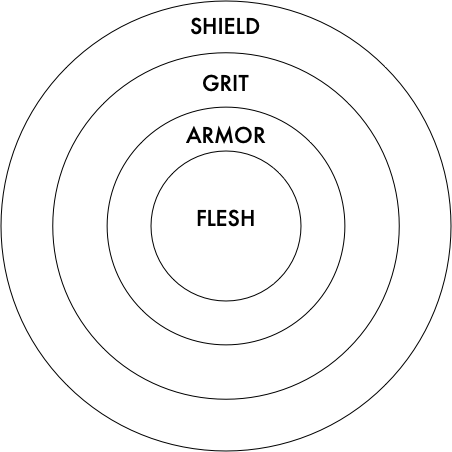
\includegraphics[scale=.3]{THE_ORDER}
  \end{center}

  \mynumlist {
    \item \mybold{Shield} : If you have a shield equipped (that is, on your arm) and take \mybold{physical damage}, and you haven't taken a Combat Action yet, you can \mylink{Splinter}{combat-deeds-splinter} your shield. Stop here.  Otherwise ...
    \item \mybold{Grit} : Subtract the damage from your Grit.  If there's any damage left over, move to Armor i.e. if I have a Grit of 4 and I take 9 damage, I have 5 damage left over and I move on to to Armor.
    \item \mybold{Armor} : If you have armor, see how much damage it will absorb.  Roll the \UD for your armor and subtract the result from the damage.  For example, if I'm wearing chain mail (Medium armor) I roll a d8; if I rolled a 5, I'd subtract 5 from the total damage. If there's any damage left over, move onto Flesh.  Remember your Armor is a \UD!
    \item \mybold{Flesh} : Subtract the rest of the damage from Flesh. If you go to 0 or less Flesh, you are \mylink{Dying}{combat-dying}
  }




\mysubsection{Flesh and Grit}{combat-flesh-grit}

Flesh is your ability to withstand injury; Grit is your ability to avoid injury in the first place.  Damage affects Grit first - dodging and weaving, close calls, little nicks, stunning blows, getting worn out from the fight, etc. When Grit is gone you're too exhausted to ward off physical harm and you start taking Flesh damage.

Your starting Flesh is defined by your \FLESH.  When you start your life as an Adventurer, your initial \FLESH is the \MAX of a d4, d6, d8, or d10 (the die is defined in your Trope or Species). You then roll your \VIG and, if the number on the die is higher than your initial \FLESH, your \MAX Flesh is this new number (for example, if I have a d6 \FLESH and a d8 \VIG, I start with 6 Flesh.  I then roll the d8 - if I roll a 7, my \MAX Flesh is now 7).

When you're \mylink{taking a Breather}{combat-resting-breather} or resting, you use your \FLESH to heal your \mybold{Grit} - basically patching yourself up, strapping wounds, getting yourself psyched up, that sort of thing.  

Flesh is generally pretty static; if you're ever at a point where you're taking damage to Flesh, you're getting pretty close to \mylink{Dying}{combat-dying}.


  \mysubsection{Dying}{combat-dying}

  \example {
    \RO: \FOC \PLUS \DEATH \PLUS \mybold{modifiers} 
  }


  If your Flesh ever goes to 0 or below, you are \mybold{Dying}.  Your Grit immediately drops to 0 if it isn't 0 already (you can't duck, dive, dodge, dip and dive while trying to hold your intestines in, right?) and your Flesh is set to 0.

  While your Flesh is at 0, you must roll a \DEATH at the \mylink{top of each Moment}{time-top-bottom}.  If you fail, you immediately perish.  You can't do anything but crawl to safety and hold your intestines in.

  Unless noted in their Trope or Species, all Adventurers' \DEATH starts at a d3.  Additional levels of \DEATH can be learned during advancement.


  \mytable{X c}{
    \thead{\DEATH} & \thead{\STATIC} \\
  }{
      Precarious & d3 \\
      Tough & d6  \\
      Resilient & d10 \\
      Enduring & d16 \\
      Amaranthine & d24 \\
  }

  The Arbiter may add negative modifiers to your roll.  A good rule of thumb for "heinous" damage (damage well in excess of your Flesh) is to divide \MAX Flesh into the result (rounded) down, and apply that as a negative modifier.  For instance, if an adventurer had 8 Flesh and took 30 damage, their roll would be at -2 (30-8 = 22.  22/8 = 2.75, rounded down = 2).

  If you are Dying, you can't heal Grit.  The moment you are healed above 0 Flesh (through Resting, Leechcraft, etc) you are no longer Dying; you must immediately roll on the \mylink{Wound table}{appendixa-combat-tables-wounds} as well as \RS : Sanity.  Note that some Wounds will prevent you from healing Grit until they are dealt with.


  \newpage
 

  \mysection{When The Dust Settles}{combat-resting}


  \mysubsection{Taking a Breather (Minutes)}{combat-resting-breather}

  Combat takes Minutes to finish, no matter how many Moments actually occurred.  Once Combat is over, you can take a \mybold{Breather}.  Roll your \FLESH and restore that much Grit up to your \MAX (unless a Wound prevents you from doing so). Pooka can help with this process significantly.  If you have \mylink{Second Skin}{sellsword-virtue-second-skin}, you can repair a \UD of Armor as well, up to its \MAX.

  You don't need to take a Breather in a safe place, but common sense should prevail - taking a quick nap in front of the goblin horde after you beheaded the chieftain isn't OK.  You can only take 1 Breather per Combat.


  \mysubsection{Taking a Bivouac (Hours)}{combat-resting-bivouac}

  If you need a longer rest, you can set up camp and take a Bivouac.  You can only camp in a "safe" place (though this doesn't necessarily have to be in \mylink{Civilization}{civilization}).  Each time you make a Bivouac, make a \UD roll of your Personal Provisions (you can share Personal Provisions with others, but you have to roll for each person).  If you don't have enough Personal Provisions, you can't get any of the good effects.  There's always a chance of wandering Monsters when you're camping, unless you have a Pooka with you


  \mybold{If a Wound doesn't prevent you from doing so:}

  \mybullet {
    \item Restore all your Grit.  
    \item Restore \LVL Flesh
    \item Restore 1 \UD of any \myital{one} \mylink{Intangible Stat}{intangible-stats}
    \item Restore your Armor up to its \MAX \UD
  }

  \cbreak

  \mybold{Additionally:}

  \mybullet {
    \item \mylink{Sellswords}{trope-sellsword} restore 1 \UD of their \DEED
    \item \mylink{Knaves}{trope-knave} and \mylink{Pooka}{species-pooka} restore 1 \UD of their Luck
    \item \mylink{Philosophers}{trope-philosopher} restore 1 Blood \POOL and/or reset any negative modifiers to Knowledge
    \item \mylink{Mystics}{trope-mystic} restore 1 Grace \POOL and/or 1 Mojo \UD
    \item \mylink{Spriggan}{species-spriggan} restore 1 Remembrance die
  }


  \mysubsection{Taking a Vacation (Days/Weeks)}{civilization-vacation}

  As your injuries mount and your experience grows,  you may find you need to take a longer rest.  Longer rests require \mylink{Civilization}{civilization}.

} %end
